%header and footer for separate chapter files

\ifx\whole\undefined
\documentclass[12pt, leqno]{book}
\usepackage{graphicx}
\input style-for-curves.sty
\usepackage{hyperref}
\usepackage{showkeys} %This shows the labels.
%\usepackage{SLAG,msribib,local}
%\usepackage{amsmath,amscd,amsthm,amssymb,amsxtra,latexsym,epsfig,epic,graphics}
%\usepackage[matrix,arrow,curve]{xy}
%\usepackage{graphicx}
%\usepackage{diagrams}
%
%%\usepackage{amsrefs}
%%%%%%%%%%%%%%%%%%%%%%%%%%%%%%%%%%%%%%%%%%
%%\textwidth16cm
%%\textheight20cm
%%\topmargin-2cm
%\oddsidemargin.8cm
%\evensidemargin1cm
%
%%%%%%Definitions
%\input preamble.tex
%\input style-for-curves.sty
%\def\TU{{\bf U}}
%\def\AA{{\mathbb A}}
%\def\BB{{\mathbb B}}
%\def\CC{{\mathbb C}}
%\def\QQ{{\mathbb Q}}
%\def\RR{{\mathbb R}}
%\def\facet{{\bf facet}}
%\def\image{{\rm image}}
%\def\cE{{\cal E}}
%\def\cF{{\cal F}}
%\def\cG{{\cal G}}
%\def\cH{{\cal H}}
%\def\cHom{{{\cal H}om}}
%\def\h{{\rm h}}
% \def\bs{{Boij-S\"oderberg{} }}
%
%\makeatletter
%\def\Ddots{\mathinner{\mkern1mu\raise\p@
%\vbox{\kern7\p@\hbox{.}}\mkern2mu
%\raise4\p@\hbox{.}\mkern2mu\raise7\p@\hbox{.}\mkern1mu}}
%\makeatother

%%
%\pagestyle{myheadings}

%\input style-for-curves.tex
%\documentclass{cambridge7A}
%\usepackage{hatcher_revised} 
%\usepackage{3264}
   
\errorcontextlines=1000
%\usepackage{makeidx}
\let\see\relax
\usepackage{makeidx}
\makeindex
% \index{word} in the doc; \index{variety!algebraic} gives variety, algebraic
% PUT a % after each \index{***}

\overfullrule=5pt
\catcode`\@\active
\def@{\mskip1.5mu} %produce a small space in math with an @

\title{Personalities of Curves}
\author{\copyright David Eisenbud and Joe Harris}
%%\includeonly{%
%0-intro,01-ChowRingDogma,02-FirstExamples,03-Grassmannians,04-GeneralGrassmannians
%,05-VectorBundlesAndChernClasses,06-LinesOnHypersurfaces,07-SingularElementsOfLinearSeries,
%08-ParameterSpaces,
%bib
%}

\date{\today}
%%\date{}
%\title{Curves}
%%{\normalsize ***Preliminary Version***}} 
%\author{David Eisenbud and Joe Harris }
%
%\begin{document}

\begin{document}
\maketitle

\pagenumbering{roman}
\setcounter{page}{5}
%\begin{5}
%\end{5}
\pagenumbering{arabic}
\tableofcontents
\fi


\chapter{Curves of genus 0 }\label{genus 0 chapter}\label{3a}\label{genus 0 and 1 chapter}

We
begin our project of describing curves in projective space with the
simplest case, 
that of
genus 0.
Even here, there are interesting
statements to make about the geometry of their embeddings in $\PP^r` `$,
and there are many open problems. 
Though we won't treat such questions, curves of genus $0$ over other fields pose their own interesting problems: the study of such curves
over $\QQ$ was a major part of 
\blue{Gauss's}
work.
\index{Gauss, Leonhard}%
\index{genus 0!curves of}%

Using Theorem~\ref{characterization of P1} and the 
\blue{Riemann--Roch theorem,}
\index{Riemann--Roch theorem}%
we can show that (over an algebraically closed field) $\PP^1$
is the only curve of arithmetic genus 0:

\begin{corollary}
 Every reduced irreducible projective curve $C$ of arithmetic genus~$0$
over an algebraically closed field is isomorphic to $\PP^1` `$.
\unif
\end{corollary}

\begin{proof}
The curve $C$ is smooth since otherwise its normalization would have negative genus.
By the Riemann--Roch theorem, any linear series $\cL$ of degree $d$ on $C$ has $h^0(\cL) \geq d+1$, so we may use Theorem~\ref{characterization of P1}
to conclude that $C\cong\nobreak \PP^1` `$.
\unif
\end{proof}

Even images of genus 0 curves must have genus 0. The following proof works as well if we replace $\CC$ by any algebraically
closed field.

\begin{npt}
\begin{theorem}[\cite{Luroth}]\label{Lueroth}
\begin{enumerate}
\item If $C\to D$ is a nonconstant map of reduced, irreducible projective curves, then the geometric genus of $C$ must be at least that of $D$.
\index{L\"uroth!Jacob}%
In particular, if $C$ has geometric genus \0,  
then 
so does
$D$.
 \item If $K$ is a field with $\CC \subsetneq K \subset \CC(x)$
  then $K = \CC(y)$ for some $y \in \CC(x)$. 
\unif
\end{enumerate}
\end{theorem}
\end{npt}

\begin{proof}
\noindent (1) Normalizing, we get a map  $ \tilde C \to \tilde D$, and
the first statement follows from 
\blue{Hurwitz's theorem.}
\index{Hurwitz's theorem}%

\smallbreak

\noindent (2) Since $\CC$ is algebraically closed, 
$K$ is a 
\blue{transcendental extension.}
\index{transcendental extension}%
\vadjust{\allowbreak}%
Since $\CC(x)$ has
transcendence degree 1, if $z\in K\setminus \CC$
then $x$ is algebraic over $\CC(z)$. Thus $\CC(x)$ is finite over $\CC(z)$, so $K$ is finite over $\CC(z)$
as well. In particular, $K$ is finitely generated over $\CC$. It follows that $K$ is the field of rational functions
on a curve $D$, and the inclusion $K\subset \CC(x)$ corresponds to a finite map $\PP^1\to D$. Applying
part (1),
we see that $D\cong \PP^1$ so $K \cong \CC(y)$ for some $y$.
\end{proof}
 
\begin{fact}[(rational curves over other fields)]
\emph{L\"uroth's theorem} refers to statement (2) in Theorem \ref{Lueroth}.
\index{L\"uroth's theorem}%
For an elementary proof of it, valid over any
field, see 
\cite[Section 8.13]{JacobsonII}.

There is an analogue 
of the last statement of part (1) of Theorem \ref{Lueroth}
for rational surfaces,
proved
by 
\index{Castelnuovo, Guido}%
Castelnuovo: every complex surface admitting a dominant rational
map from $\PP^2$ is rational (see \cite[Corollary V.5]{Beauville}, for
example). 
However, the analogue in higher 
dimensions
is false; for example, \cite{MR0302652} shows that a smooth cubic threefold $X$ admits a dominant rational map $\PP^3 \to X$ but is not rational.

Over a nonalgebraically closed field, a curve $C$ of genus 0 need not
have any points, or any line bundles of odd degree. Since the
canonical bundle $K_C$ has degree $-2$, there do necessarily exist
line bundles of every even degree; thus an arbitrary curve of genus 0
is isomorphic to a  
\blue{plane conic.}
\index{plane conic}%

A projective curve of genus 0 over a field $k$ is called a 
\,\emph{form} 
\index{form of $\PP\sp1$}%
of $\PP^1$ if it becomes isomorphic to $\PP^1$ after extension
of scalars to
the algebraic closure of $k$. The unique example with $k = \RR$ that
is not isomorphic over $\RR$ to $\PP^1$
is the conic with no $\RR$-rational points, $x^2+y^2+z^2 = 0$. 

Noncommutative algebras enter the subject of forms of $\PP^1$ (and
$\PP^n$ more generally) in a surprising way: The curve $\PP_k^1$
itself may be described as the scheme of 
\index{left ideals!scheme of}%
left ideals of $k$-vector-space dimension 2 in the ring of
$2\times 2$ matrices over $k$: such an ideal can be embedded in the
matrix ring as a linear combination of the 2 columns in an appropriate sense. 
More generally, any scheme that is a form of $\PP^1$ over $k$
may be described as the scheme of 2-dimensional left ideals in a 
4-dimensional central simple ($=$ 
\blue{Azumaya) algebra}
\index{Azumaya algebra}%
over $k$. For example, the
conic $x^2+y^2+z^2 = 0$ with no points over $\RR$ is the scheme of 
left ideals in the algebra of 
\blue{quaternions.}
\index{quaternions}%
See \cite[Section X.6]{Serre1979}.
\end{fact}

\section{Rational normal curves}\label{rational normal curves section}

\subsubsection*{The homogeneous coordinate ring of a rational normal curve}

If $\sV = (V,\sL)$ is a linear series on a scheme $X$, then the inclusion
$V\subset H^0(\sL)$ induces by multiplication a map
$$
\rho_{\sV}: \Sym(V) \to  \bigoplus_{n\in \ZZ} H^0(\sL^n)
$$
from the symmetric algebra of $V$.
\marginpar{moved}
When $\sV$ embeds $X$ in $\PP^r = \PP V` `$, the image $R_{X}$ of this map is called the \emph{homogeneous coordinate ring} of $X$. 
\index{homogeneous coordinate ring}%
\index{coordinate ring!homogeneous}%

The 
\blue{rational normal curve}
\index{rational normal curve}%
$C\subset \PP^d$ of degree $d$ is embedded by the complete linear series
$\sV = (\sO_{\PP^1}(d), \CC[s,t]_d)$. Since any form of degree $nd$ in $\CC[s,t]$ is a sum of products of $n$ forms of degree $d$, 
the corresponding homogeneous coordinate ring of the rational normal curve is 
$$
\CC[s,t]_{(d)} := \bigoplus_n(\CC[s,t]_{nd}),
$$
and the map $\rho_{\sV}$ is surjective. This is expressed by saying
that $C$ is 
\blue{\emph{arithmetically Cohen--Macaulay};}
\index{ACM}%
\index{arithmetically Cohen--Macaulay}%
more generally, if $C\subset \PP^r$ is 
\index{linearly normal}%
\index{quadratically normal}%
\index{normal!linearly / quadratically / $n$-ically}%
a one-dimensional scheme, we say that $C$ is linearly (respectively, quadratically, \dots, $n$-ically) normal
if  the natural maps
$$
\rho_m: H^0(\sO_{\PP^r}(m)) \to H^0(\sO_{C}(m))
$$
are surjective for  $m=1$ (respectively $m=2,\dots, m=n$). We say that $C$ is arithmetically Cohen--Macaulay
(usually abbreviated ACM)
 when $\rho_m$ is surjective for all $m$. We'll discuss the
 significance of this condition in Section~\ref{ACM},
and we will prove that it is equivalent to the condition 
that $R_{C}$ is a Cohen--Macaulay ring, justifying
\index{Cohen--Macaulay ring}%
 the name.



\subsubsection*{The equations defining a rational normal curve}

Choosing a basis $s,t$ for the linear forms on $\PP^1` `$, we can
write the $d$-th 
\index{Veronese map}%
Veronese map $\PP^{1}\to \PP^{d}$ as
$$
\phi_d : (s,t) \mapsto (s^d, s^{d-1}t,\dots, t^d)
,
$$
from which we see that the image $C$ of $\phi_d$ lies in the zero locus of the homogeneous quadratic polynomial $x_i x_j - x_{i+1}x_{j-1}$ for every $i,j$. We can realize these quadratic forms as the $2\times 2$ minors of the matrix
$$
M \; = \; \begin{pmatrix}
x_0 & x_1 & \dots & x_{d-1} \\
x_1 & x_2 & \dots & x_d
\end{pmatrix}.
$$
Note that if we substitute $s^it^{(d-i)}$ for $x_i$ and identify $H^0(\cO_{\PP^1}(i))$ with $\CC[s,t]_i$, this becomes the multiplication table
$$
H^0(\cO_{\PP^1}(1)) \times H^0(\cO_{\PP^1}(d{-}1)) \to H^0(\cO_{\PP^1}(d)).
$$


It is easy to see that $C$ is 
set-theoretically 
\index{set-theoretic equality}%
\index{minors, $2\times 2$}%
defined by the $2\times 2$ minors of $M$: the affine set $s=1$ in $\PP^1$ maps
to the affine set $x_0 = 1$ in $\PP^d` `$, and the affine form of the map is $t \mapsto (t, t^2, \dots, t^d)$. But if $x_1 = t$ then from 
the equations $x_0x_i = x_1x_{i-1}$ we see successively that $x_i = t^i$; 
that is, the vanishing of the minors of $M$ at a point $p$
implies that $p$ lies on $C$.

A much stronger statement is true:

\begin{proposition}\label{RNC generators} The homogeneous ideal of the
\blue{rational normal curve}
\index{rational normal curve}%
$$
\PP^1 \rOnto C \subset \PP^d,\quad (s,t) \mapsto (s^d, s^{d-1}t, \dots, t^d),
$$ 
 is generated by the
 $2\times 2$ minors of $M$.
  \end{proposition}
  
% By way of notation, we write
% $\CC[s,t]_{(d)}$ for the subring of $\CC[s,t]$ generated by all forms whose degree is a multiple of $d$. 
% Since any monomial of degree $nd$ is a product of $n$ monomials of degree $d$, the map
% $$
% \Sym^d H^0(\sO_{\PP^1}(n)) \to H^0(\sO_{\PP^1}(nd)) = \CC[s,t]_{nd}
% $$
% corresponding to $\phi_d$ is surjective, so $\CC[s,t]_{(d)}$ is the homogeneous coordinate ring of $C$,
% and the Proposition amounts to saying that $\CC[x_0,\dots, x_d]/I \cong \CC[s,t]_{(d)}$.
% 
 
\begin{proof}
Let $I\subset \CC[x_0,\dots, x_d]$ be the ideal generated by the $2\times 2$ minors of $M$.
As we have seen, the map
$$
\phi: \CC[x_0, \dots, x_d]/I \rOnto \CC[s,t]_{(d)},\quad x_i\mapsto s^{d-i}t^i,
$$
is surjective, and we must show that this is a monomorphism, or equivalently that the source of $\phi$ in degree $n$ has
(at most) the same dimension $nd+1$ as the target of $\phi$ in degree $nd$.

If $0<i\leq j<d$ then 
$$
x_ix_j \equiv x_{i-1}x_{j+1}  \ (\mathrm{ mod}\ I).
$$
Thus every monomial in the $x_i$ of degree $t$ is equivalent, modulo $I$, to a monomial of the form
 $$
 x_0^ax_1^{\epsilon_1}\cdots x_{d-1}^{\epsilon_{d-1}}x_d^b
 $$
 where at most one $\epsilon_i$ is 1, and the rest are 0. There are $n+1$ such elements of degree $n$ with all the $\epsilon_i = 0$
 and $n(d-1)$ elements with one of the $\epsilon_i = 1$. Thus there are $nd+1$ such elements in all, proving that $\phi$ is
 an isomorphism.
  \end{proof}

\begin{fact}\label{Veronese equations fact}
The description of the equations above can be considerably extended;
see Proposition~\ref{some equations}. For example, the equations of the 
\index{Veronese surface}%
Veronese surface, which is the image of $\PP^{2}$
 under the complete linear system of quadrics, is defined by the $2\times 2$ minors of the generic
 symmetric matrix 
 $$
 \begin{pmatrix}
 x_{0}&x_{1}&x_{2}\\
  x_{1}&x_{3}&x_{4}\\
   x_{2}&x_{4}&x_{5}\\
\end{pmatrix}
,
$$
which arises from the multiplication table of 
\belowdisplayskip-\baselineskip
$$
H^{0}(\sO_{\PP^{2}}(1)) \otimes H^{0}(\sO_{\PP^{2}}(1)) \to H^{0}(\sO_{\PP^{2}}(2)).
$$
\end{fact}

\vspace*{3pt}

\begin{corollary}\label{forms vanishing on the RNC}
The dimension of the degree $n$ part of the homogeneous ideal of the 
\blue{rational normal curve}
\index{rational normal curve}%
of degree $d$ is
$$
H^0(\sI_{C/\PP^d}(n)) = \mbinom{n+d}{n} - (nd+1).
$$
In particular 
\end{corollary}

\begin{proof}
The 
\blue{homogeneous coordinate ring}
\index{homogeneous coordinate ring}%
of the rational normal curve is 
$$\CC[s,t]_{(d)}\subset \CC[s,t].$$ 
Comparing the dimension
of $\CC[x_0,\dots,x_d]_n$ with the dimension of $\CC[s,t]_{nd}$ gives the result.
\end{proof}

The number of quadrics containing the
\blue{rational normal curve}
\index{rational normal curve}%
is extremal:
\index{extremal number of quadrics}%
\index{number!of quadrics containing the rational normal curve}%

\begin{proposition}\label{rnc on most quadrics}
If $C \subset \PP^d$ is any irreducible, nondegenerate curve, then
$$
h^0(\cI_{C/\PP^d}(2)) \leq  \mbinom{d}{2}.
$$
Equality holds only if
$C$ is a rational normal curve.
\unif
\end{proposition}

In the proof we will use a general fact about hyperplane sections:
\index{hyperplane sections}%

\begin{proposition}\label{arbitrary hyperplane}
If $\,X\subset \PP^r$ is a nondegenerate, reduced, irreducible variety, 
then $H^0(\sI_X(1)) = H^1 (\sI_X) = 0$. 
Moreover if $H$ is any hyperplane of $\PP^r` `$, defined by
a linear form $h$, then the natural
sequence
$$
0\to \sI_{X/\PP^r} \ruto {\ h} \sI_{X/\PP^r}(1)\to \sI_{(H\cap X)/H}(1)\to 0
$$
arising from the restriction of the ideal sheaf $\sI_{X/\PP^r}$ to $H$ is exact, and the subscheme
$H\cap X$ spans $H$; that is, $H^0(\sI_{(H\cap X)/H}(1)) = 0$.
\unif
\end{proposition}

See Exercise~\ref{arbitrary hyperplane examples} for the necessity of the hypotheses
and Exercise~\ref{restriction of ideals} for a generalization. 

\begin{corollary}\label{minimal degree bound}
If $X\subset \PP^r$ is a nondegenerate, reduced, irreducible variety of codimension $c$, then $\deg X \geq c+1$.
\unif
\end{corollary}

\begin{proof}
 The intersection of $X$ with a general plane $\Lambda$ of dimension $c$ is a finite scheme spanning $\Lambda$.
\unif
\end{proof}
%Note that
%${H\cap X}$ could have embedded components of dimension $<\dim X -1$, though in the case where $X$ is a curve
%this is obviously impossible. 

\begin{proof}[Proof of Proposition~\ref{arbitrary hyperplane}]
Since
$X$ is reduced, irreducible and  \null nondegenerate,
$h$ is a nonzerodivisor modulo 
$\sI_{X/\PP^r}@$, so $h\sI_{X/\PP^r} = (h)\cap \sI_{X/\PP^r}$ where
$(h) = h\sO_{X}$. 
Setting $\Gamma = {H\cap X}$
we have 
$$
\begin{aligned}
\sI_{X/\PP^r}(1)/h\sI_{X/\PP^r} &= \sI_{X/\PP^r}(1)/((h)\cap\sI_{X/\PP^r})\\
 &=(\sI_{X/\PP^r}(1)+(h))/(h)\\
 &= \sI_{\Gamma/H}(1),
\end{aligned}
$$
from which the exactness assertion follows.
 
 Again because $X$ is reduced and irreducible, $H^0(\sO_X)$ contains only the constant function, so the map $H^0(\sO_{\PP^r}) \to H^0(\sO_X)$ is surjective, 
from which it follows that $H^1(\sI_{X/\PP^r}) = 0.$ From the long exact sequence in cohomology it follows that
 the restriction map $H^0(\sI_{X/\PP^r}(1))\to H^0(\sI_{\Gamma/H}(1))$ is surjective. Since
$X$ is nondegenerate, $H^0(\sI_{X/\PP^r}(1)) = 0$, and the desired result follows.
\unif
\end{proof}


\begin{proof}[Proof of Proposition~\ref{rnc on most quadrics}]
Consider the restriction of the quadrics containing $C$ to a general hyperplane $H \cong \PP^{d-1} \subset \PP^d` `$, and let $\Gamma = H \cap C$. There is an exact sequence:
$$
0 \to \cI_{C/\PP^d}(1) \to \cI_{C/\PP^d}(2) \to \cI_{\Gamma/\PP^{d-1}}(2) \to 0.
$$ 
Proposition~\ref{arbitrary hyperplane} shows that $h^0(\cI_{C/\PP^d}(1)) = h^1(\cI_{C/\PP^d}(1))=0$, so $\Gamma$
imposes the same number of conditions on quadrics as $C$ does.

Proposition~\ref{arbitrary hyperplane} also shows that $H$ is the
\vadjust{\allowbreak}%
linear span of  $\Gamma$. 
Therefore
the hyperplane section $\Gamma$ of $C$ must contain at least $d$
linearly independent points (this gives another proof that 
such a curve must have degree $\geq d$.)
Any set of linearly independent points imposes independent conditions on linear forms, and thus also on quadrics (see 
Proposition~\ref{min hilb} for a stronger result). 
Thus
$$
h^0(\cI_{\Gamma/\PP^{d-1}}(2)) \leq h^0(\cO_{\PP^{d-1}}(2)) - d = 
\mbinom{d+1}{2} - d = \mbinom{d}{2},
$$
establishing the desired inequality. 

To prove that 
equality can be achieved only with the rational normal curve, 
suppose that $C\subset \PP^{d}$
is not a rational normal curve, so that $\deg C >d$. Let
$$
\Gamma' \subset H \cong \PP^{d-1}
$$
be a subset 
of $d$ linearly independent points of a general hyperplane section $H\cap C$
and let $\Gamma = \Gamma'\cup\{p\}\subset H$ be a subset containing one more point.

We will
show that $p$ imposes a nontrivial vanishing condition on quadrics containing $\Gamma'$, since
then $C$ 
will lie
on fewer quadrics than the rational normal curve.
Since the points of $\Gamma'$ are linearly independent, each subset of
$d{-}1$ of them spans a $(d{-}2)$-plane inside $H$, and the intersection
of these spans is empty. Thus one of the spans $\Lambda$ does not
contain $p$. 
The union of  a general hyperplane $H$ containing $\Lambda$ and a general hyperplane containing 
the point $\Gamma' \setminus \Gamma'\cap \Lambda$
is a quadric containing $\Gamma'$ but not $p$, as required. 
\unif
\end{proof}

For each $m$, rational normal curves lie on more hypersurfaces of degree $m$ than any other irreducible, nondegenerate curve in $\PP^d`$; see Exercise~\ref{extremal m-ics}.

\subsubsection*{Rational normal curves are projectively homogeneous}

An
important property of rational normal curves $C \subset \PP^d$
is that they are \emph{projectively homogeneous},
in the sense that the
subgroup $G\subset\PGL_{d+1}$ of automorphisms of $\PP^d$ that carry
$C$ to itself acts transitively on $C$. More generally: 
\index{projectively homogeneous}%

\begin{proposition}\label{Veronese is projectively homogeneous}
If $@X\subset \PP^n$ is the image of $\,\PP^r$ by the Veronese map 
\index{Veronese map}%
associated
to $|\sO_{\PP^r}(d)|$, then $X$ is projectively homogeneous.
\unif
\end{proposition}

\begin{proof}
$\PP^r$ 
itself
is a homogeneous variety
in that $\Aut \PP^r$ acts transitively. 
For any
automorphism 
$\sigma$ of $\PP^r$, we have
$\sigma^*\cO_{\PP^r}(d) = \cO_{\PP^r}(d)$
because $\cO_{\PP^r}(d)$ is the unique
invertible sheaf of degree $d$ on $\PP^r` `$;  
thus
$\sigma$ induces an automorphism $\phi$ on $H^0(\cO_{\PP^r}(d))$ 
and an automorphism $\bar \phi$ on the ambient space 
$\PP^{N} := \PP H^0(\cO_{\PP^r}(d))$ of the target of the $d$-th Veronese map. If $\ell \in H^0(\cO_{\PP^r}(d))$
 with divisor $D\subset X$, then $\phi(\ell) = \ell \circ \sigma$ has divisor $\sigma^{-1}(D)$, so $\bar\phi^{-1}$ induces $\sigma$ on $\PP^r` `$. 
\unif
\end{proof}

The
\blue{rational normal curve}
\index{rational normal curve}%
$C \subset \PP^d$ can  be characterized among irreducible,
nondegenerate curves as the unique projectively homogeneous curve in
$\PP^d$ (Corollary~\ref{uninflected curves}).

\subsubsection*{%
{\color{blue}Interpolation}  %\blue
for rational normal curves}
\index{interpolation!of $d+3$ points}%

Another 
striking
property of rational normal curves is expressed in
the following 
proposition.
Recall that a collection of points (or a finite subscheme)
of $\PP^d$ is 
\emph{in linearly general position} 
if no $k{+}1$ of them lie in a $(k{-}1)$-plane with $k\leq n$. 

\begin{proposition}\label{points on rnc}
\index{linearly general position}%
Any $d+3$ points $p_1,\dots, p_{d+3} \in \PP^d$ 
in linearly general position
lie on a unique rational normal curve $C \subset \PP^d$.
\unif
 \end{proposition}

\begin{proof}
There is an automorphism $\Phi : \PP^d \to \PP^d$ carrying 
$p_1,\dots,p_{d+1}$ to the coordinate points
$(0,\dots,0,1,0,\dots,0)\in \PP^d$ and the point $p_{d+2}$ to the
point $(1,1,\dots,1)$.  Denote the image of the remaining  point
$p_{d+3}$  by $[\alpha_0,\dots,\alpha_n]$. We consider maps $\PP^1 \to
\PP^d$ given in terms of an inhomogeneous coordinate $z$ on $\PP^1$ by
$$
z \mapsto \left( \frac{1}{z - \nu_0}, \frac{1}{z - \nu_1} , \dots, \frac{1}{z - \nu_d}  \right)
$$
with $\nu_0,\dots,\nu_d$ any distinct scalars. Clearing denominators,
we see that the image of such a map is a rational normal curve, and it
passes through the $d+1$ coordinate points of $\PP^d` `$, which are
the images of the points $z = \nu_0, \dots, \nu_d \in \PP^1` `$. 
Moreover, the image of the point  at infinity is $(1,1,
\dots,1)$. Because the points are assumed linearly independent, the
$\alpha_i$ must all be nonzero, and thus if we take  $\nu_i =
-1/\alpha_i$, the image of the point $z = 0$ is
$(\alpha_0,\dots,\alpha_d)$. This proves existence; we leave
uniqueness to Exercise~\ref{Castelnuovo uniqueness}.
\unif
\end{proof}

\begin{fact}
A generalization of Proposition~\ref{points on rnc} is given, with a proof that is different
even in our case, in \cite[Proposition 3.19]{Montreal}.  There is also a version replacing the set of $d+3$ distinct points by a  finite
scheme of degree $d+3$ satisfying necessary conditions, in \cite{EHLGP}.
\end{fact}

Given some ``natural''
family of curves in projective space $\PP^r$ (such as an open set of smooth
curves in a component of the Hilbert scheme 
described in Chapters
\ref{ModuliChapter} and \ref{HilbertSchemesChapter}) 
and an integer $m$, we can ask whether there exists a curve in the
family passing through $m$ given general points of $\PP^r` `$. 
Proposition~\ref{points on rnc}
gives the only example we know of curves other than complete
intersections for which there is a \emph{unique} such curve.

\section{Other rational curves}

What about other rational curves in projective space? 

Any linear series $\cD$ of degree $d$ on $\PP^1$ is a subseries of the complete series $|\cO_{\PP^1}(d)|$, so any map $\phi : \PP^1 \to \PP^r$ of degree $d$ may be given as the
composition of the embedding $\phi_d : \PP^1 \to \PP^d$ of $\,\PP^1$
as a rational normal curve with a linear projection $\pi : \PP^d \to
\PP^r` `$. Since the natural degree $d$ 
\blue{Veronese embedding}
\index{Veronese embedding}%
of $\PP^1 =
\PP(V)$ as the rational normal curve is the map
$\PP V \to \PP(\Sym^d(V))$, the projection is a map into $\PP W` `$, where $W\subset \Sym^d(V)$. 

We can make this more explicit in several ways: first, choosing a basis $s,t$ for $V$ and a basis of forms $F_i$ of degree $d$ on $\PP^1$ for $W` `$, we may write the map as
$$
(s,t) \; \mapsto \; \left(F_0(s,t), \dots, F_r(s,t)\right).
$$
If the $F_i$ have a greatest common factor $G(s,t)$ then the set $G=0$ will be the base locus
of the linear series, and the map
$$
(s,t) \; \mapsto \; \left( \frac{F_0(s,t)}{G(s,t)}, \dots, \frac{F_r(s,t)}{G(s,t)}\right).
$$
gives the same map, represented as a linear series of lower degree $d-\deg G$. Thus we
will now assume that the forms in $W$ have no common factor.

\begingroup \let\;\,
Perhaps 
more simply,
we can pass to an open affine 
$\AA^1\subset\PP^1$
given by $t=1$, 
with coordinate function $z = s/t$, and
dehomogenize the $F_i$ to get a vector space of polynomials $f_i = F(s,1)$ of degree $\leq d$. Then we may write the
map as
$$
z \; \mapsto \; (f_0(z), \dots, f_r(z)).
$$
Since the $F_i$ have no common factor, and 
thus
are not all divisible by $t$, at least one of the
$f_i$ will have degree exactly $d$.
For example, the twisted cubic itself can be represented by the map
$z \mapsto (1, z,z^2,z^3)$.

Here, we think of a polynomial $f(z) = f(s/t)$ of degree $\leq\ d$ 
as a rational function on $\PP^1$ having
a pole of order at most $d$ at the point at infinity $(1,0)\in \PP^1`$; but we could also take rational
functions $F_i(s,t)/G_i(s,t)$ of total degree $\deg F_i-\deg G_i = d$ or, dehomogenizing, $\phi_i(z) = f_i(z)/g_i(z)$.

\subsection*{Smooth rational quartics}

Given how easy it is to describe rational curves in projective space
\index{rational quartics}%
in this way, it is surprising how many open questions there are. We
begin with 
one of the simplest cases: a smooth nondegenerate rational curve $C$ of degree $4$ in $\PP^3` `$.
As described above, such a curve is the image of $\PP^1$ under a map given by 4 quartic forms,
or, in the most coordinate-free formulation, a codimension 1 subspace of $\Sym^4(V)$, where
$V\cong \CC^2` `$. 

\begin{example}
In Exercise~\ref{distinguishing rational quartics} the reader 
is asked to
prove that there is a 1\hbox{-}parameter family of 
$\PGL_4$ orbits of smooth rational quartic curves in $\PP^3` `$. 
Perhaps the simplest is given by the parametrization 
$$
\PP^1 \ni (s,t) \mapsto (s^4, s^3t, st^3, t^4)\in \PP^3,
$$
or, more simply, $t\mapsto(t, t^3, t^4)$. 

Proposition~\ref{ideal of rational quartic} shows that the homogeneous
ideal of this curve requires~4 generators, and it is not hard to show
that the ideal is generated scheme theoretically (that is, up to saturation) by 3 elements. Nevertheless it is
one of the most famous open problems in the theory of curves to determine whether or not the ideal
is generated up to radical by just 2 elements\emdash that is, whether it
can be written 
\emph{set-theoretically} 
\index{set-theoretic equality}%
as the intersection of two surfaces. For a sample of the recent
work on this, see \cite{MR3356940}. 
\end{example}

\begin{proposition}\label{ideal of rational quartic}
If $C\subset \PP^3$ is a smooth rational quartic curve, then $C$ lies on a smooth quadric
surface $S$ in the divisor class $(1,3)$, and the homogeneous ideal of $C$ is minimally
generated by the quadric defining $S$ and three cubic forms.
\end{proposition}

\begin{proof}
We first consider the restriction maps
$$
\rho_e: H^0(\op3e)\to H^0(\cO_C(e)).
$$
Since $C\cong \PP^1` `$,
we may identify $H^0(\cO_C(e))$ with 
$H^0(\op1{4e})$.
 Since we assume that $C$ is nondegenerate, it does not lie on a hyperplane,
 so  $\rho_1$ is a monomorphism. 
 
The source $H^0(\op32)$ of $\rho_2$ is 10-dimensional, and the target $H^0(\op18)$ is
9-dimensional, so $\rho_2$ has a kernel of dimension at least 1; that is, $C$ lies on
a quadric surface, and since $C$ is irreducible and nondegenerate, any quadric surface containing
$C$ is irreducible. This quadric is smooth; 
see Example~\ref{curve on rank 3 quadric}.

%If $C$ lay on a second quadric surface, then, since the quadrics must be irreducible,
%$C$ would be contained in the complete intersection of the two, which also has degree 4, so 
%$C$ would be the complete intersection of the two quadrics. But by adjunction such a curve would have genus 1, so this can't be the case (indeed, we'll encounter such curves in the next section, when we take up curves of genus 1).

Given that $C$ lies on a smooth quadric surface $Q$, we consider its divisor class $(a,b)$ in the 
Picard group $\Pic(Q) = \ZZ\oplus \ZZ$. As we saw in Example~\ref{curves on quadrics}, a smooth curve
in the class $(a,b)$ has degree $a+b$ and genus $(a{-}1)(b{-}1)$;
solving the equations $a+b=4$ 
and
$(a{-}1)(b{-}1)=0$ we see that $C\sim (1,3)$ or $C\sim (3,1)$. Since the cases
are symmetric we assume $C\sim(1,3)$. 

The source of $\rho_3$ is 20-dimensional and the target is 
13-dimensional so there are at least 7
cubics in the ideal of $C\subset \PP^3` `$. Four of these come from multiplying the quadric
by the 4 variables on $\PP^3` `$, so there are at least 3 more cubic generators in $I_{C/\PP^3}$,
 the homogeneous ideal of $C$. 

From the exact sequence 
$$
0\to I_{Q/\PP^3} \to I_{C/\PP^3} \to I_{C/Q} \to 0
$$
we see that $I_{C/\PP^3}$ is generated by the form defining the quadric 
together with generators for $I_{C/Q}$. Moreover, 
the natural inclusion $I_{C/Q}\subset H^{0}_{*}(I_{C/Q})$ is an equality; this follows from the exact sequence of sheaves
$$
0\to \sI_{Q/\PP^3} \to \sI_{C/\PP^3} \to \sI_{C/Q} \to 0
$$
because $H^{1}_{*}(\sI_{Q/\PP^3}) = H^{1}_{*}(\sO_{\PP^3}(-2)) = 0$.
Thus we need only compute generators for $H^{0}_{*}(I_{C/Q})$.

Since $C$ lies in class $(1,3)$ we see that 
$$
\sI_{C/Q}(d) = \cO_{\PP^1\times \PP^1}(d{-}1, d{-}3)
.
$$
By the K\"unneth formula,
$$
h^0(\sI_{C/Q}(3)) = h^0(\cO_{\PP^1\times \PP^1}(2, 0)) = h^0(\op12)\cdot h^0(\op10) = 3,
$$
and we see that $I(C)$ contains just 3 cubic generators modulo the quadric defining $Q$. 

We claim that the three generators of $h^0(\cO_{\PP^1\times \PP^1}(2, 0))$ generate all of
$$
H^0_{*}(\sI_{C/Q}(3)) = H^0_{*}(\cO_{\PP^1\times \PP^1}(2, 0)) = 
\tsty
\bigoplus\limits_{m\geq 0}H^{0}(\cO_{\PP^1\times \PP^1}(m+2,m)).
$$
For this we must show that the maps
$$
\rho_{m}: H^{0}(\op31) \otimes H^0(\sI_{C/Q}(m+3)) \to H^0(\sI_{C/Q}(m+1+3))
$$
are surjective for $m\geq 0$.

Since the restriction
of $H^0(\op31)$ to the quadric is 
$$
H^0(\sO_{\PP^1\times \PP^1}(1,1)) = H^{0}(\sO_{\PP^{1}}(1)) \otimes H^{0}(\sO_{\PP^{1}}(1)),
$$
the map $\rho_{m}$
is the tensor product of the two maps
$$
H^{0}(\op11)\otimes H^{0}(\op1{m+2}) \to H^{0}(\op1{m+1+2})
$$
and 
$$
H^{0}(\op11)\otimes H^{0}(\op1{m}) \to H^{0}(\op1{m+1})
,
$$
both of which are surjective for $m\geq 0$. This completes the proof.
\end{proof}

\begin{figure}
\Small
\hskip-46pt\vbox{\vskip-24pt\hbox{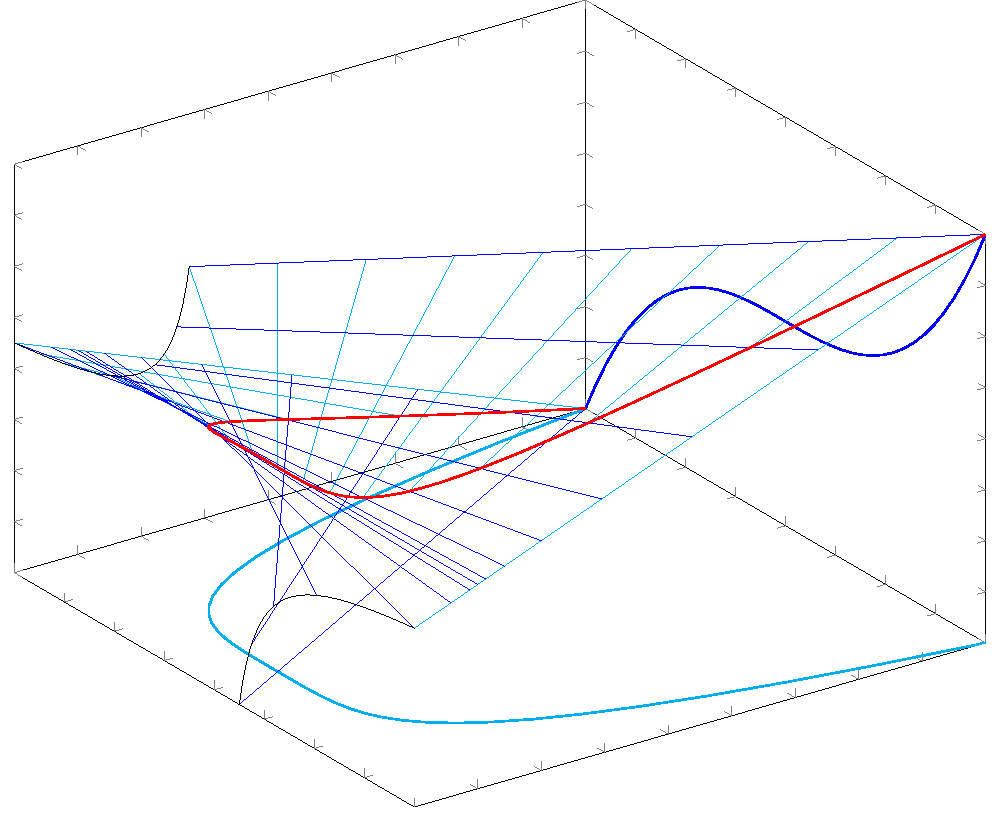
\includegraphics[scale=0.6,angle=74]{main/Fig03-newfigg}}\vskip-20pt}\hskip-50pt
%
\rlap{\hskip6pt\raise150pt\hbox{$z$}}%
\rlap{\hskip1.5pt\raise116pt\hbox{$_0$}}%
\rlap{\hskip1.5pt\raise191pt\hbox{$_{8}$}}%
\rlap{\hskip1pt\raise267pt\hbox{$_{16}$}}%
%
\llap{\raise37pt\hbox{$x$}\hskip40pt}%
\llap{\raise2pt\hbox{$_{-2}$}\hskip89pt}%
\llap{\raise24pt\hbox{$_{-1}$}\hskip66pt}%
\llap{\raise47pt\hbox{$_0$}\hskip44pt}%
\llap{\raise70pt\hbox{$_1$}\hskip20pt}%
\llap{\raise92pt\hbox{$_2$}\hskip-2pt}%
%
\llap{\raise11pt\hbox{$y$}\hskip167pt}%
\llap{\raise32pt\hbox{$_8$}\hskip210pt}%
\llap{\raise24pt\hbox{$_4$}\hskip182pt}%
\llap{\raise16pt\hbox{$_0$}\hskip152pt}%
\llap{\raise8pt\hbox{$_{-4}$}\hskip124pt}%
\llap{\raise1pt\hbox{$_{-8}$}\hskip98pt}%
%
 \caption{A rational quartic space curve $t\mapsto (t,t^3,t^4)$, shown in red, of type $(1,3)$, on a quadric surface $z=xy$,
 illustrated via  its rulings and its intersections with the bounding planes.
The red curve projects
to the dark blue curve $y=x^3$ in the $xy$-plane on the top surface of the box
 and the light blue curve $z=x^4$ on the front face.
\marginparhere{\vskip-100pt\hsize=1.5\hsize \redden{ it would be a help to 
put a text box "y=8" with an arrow pointing to the straight line that is the intersection of the quadric with the y=8 plane, and 
similarly with the intersections with the x = -2 and z = -2 planes. }}
(Inspired by code of Enrique Acosta Jaramillo for the twisted cubic.)
}
\end{figure}

\subsection*{Some open problems about rational curves}

We can say far less about rational curves of higher degree, even in $\PP^3` `$. For example, when $d$ is large, we
don't know the possible Hilbert functions for curves of degree $d$ in $\PP^3` `$, and the situation in $\PP^r$ for
$r>3$ is even worse. However, we do know the Hilbert function of a \emph{general} rational curve $C \subset \PP^r$ of degree $d$. 

Since such statements will come up often, we pause to explain 
exactly what it means to say
\index{general@a general X has property Y}%
``A general X has property Y.'' This
statement presupposes a choice of a parameter space for objects of
type X, 
that is to say, an algebraic variety $Z$ whose points each correspond to an object of type X. Thus, to be precise, the statement should be,
``An  object of type X that is general with respect to parameter space $Z$ has property Y.'' The statement then means: inside $Z$ there is
a dense open set whose elements correspond to objects of type X that have property Y. Often $Z$ is irreducible, and
then it is enough to have a nonempty open set, since every such set is Zariski dense.

In the case of nondegenerate rational curves
of degree $d$ in $\PP^{r}$ 
we could take for $Z$ the space of
$(r@{+}1)$-tuples of independent elements of $H^{0}(\op1d)$, or
equivalently, taking the quotient by $\PGL(r+1)$,
the 
\blue{Grassmannian}
\index{Grassmannian}%
 of $(r@{+}1)$-dimensional planes in $H^{0}(\op1d)$.
We will later make statements about general curves of genus $g$, referring either to 
a component of a Hilbert scheme 
(discussed in Chapter \ref{ModuliChapter}) or to the
moduli space of curves that is discussed at length in Chapter 
\ref{CurvesModuliChapter}.

As in Proposition~\ref{ideal of rational quartic}, knowing the Hilbert function of a curve $C\subset \PP^{r}$ is tantamount to knowing the ranks of the restriction maps
$$
\rho_m : H^0(\cO_{\PP^r}(m)) \to H^0(\cO_C(m)) = H^0(\cO_{\PP^1}(md)).
$$
Equivalently we ask: if $V$ is a general  $(r+1)$-dimensional vector space of homogeneous polynomials of degree $d$, what is the dimension of the space of polynomials spanned by $m$-fold products of polynomials in $V$? 

We might guess that the answer is, ``as large as possible," meaning
that the rank of $\rho_m$ is $\tbinom{m+r}{r}$ or $md+1$, 
whichever is less
\emdash in
other words, the map $\rho_m$ is either injective or surjective for
each $m$. This was proved in \cite{Ballico-Ellia83}, and is a special
case of Larson's maximal rank theorem \cite{Larson}.

As we will see in subsequent chapters it is possible to speak of a 
\index{general curve of genus $g$}%
general curve of genus $g$
and a 
\index{general invertible sheaf}%
general invertible sheaf
of degree $d$ on such a curve; and the analogous statement 
about Hilbert functions  was proven in \cite{ELarson2018}; see Chapter~\ref{Brill--Noether}.

Nevertheless, even the degrees of the generators of the homogeneous ideal of a general
rational curve of degree $d$ in $\PP^3$ is unknown for larger $d$. 

\subsubsection*{The secant plane conjecture}

If $C \subset \PP^r` `$, then an $e$-secant $s$-plane to $C$ is an
$s$-plane $\Lambda \cong \PP^s \subset \PP^r$ such that the
intersection $\Lambda \cap C$ has degree $\geq e$. 
\index{secant plane conjecture}%

Should you expect a curve $C \subset \PP^r$ to have any $e$-secant
$s$-planes? The set of $s$-planes in $\PP^r$ is parametrized by the 
\blue{Grassmannian}
\index{Grassmannian}%
$\GG = \GG(s,r)$, which has dimension $(s+1)(r-s)$. Inside $\GG$, the locus of planes that meet $C$ has codimension $r-s-1$ (reason: the locus of planes containing a given point $p$ is isomorphic
by projection from $p$ to $\GG(s-1,r-1)$, and thus has codimension $r-s$). 
Thus one might conjecture that a curve $C \subset \PP^r$ 
will have $e$-secant $s$-planes when 
\vspace*{-3pt}
$$
e \; \leq \; (s+1)\frac{r-s}{r-s-1},
$$
perhaps with a few low-degree exceptions. Is this true of a general rational curve? For most $e$, $r$ and $s$, we don't know.

\section{The Cohen--Macaulay property}\label{ACM}

In Section~\ref{rational normal curves section} we defined a curve
$C\subset \PP^{r}$ to be arithmetically Cohen--Macaulay (ACM) if the
\index{Cohen--Macaulay}%
natural maps 
$$
\rho_m: H^0(\sO_{\PP^r}(m)) \to H^0(\sO_{C}(m))
$$
are surjective for all $m$. When this is the case we can accurately predict the number of independent forms of
each degree vanishing on the curve, and the condition has other important consequences that we will explore here and in Chapters~\ref{LinkageChapter} and \ref{SyzygiesChapter}. For general treatments of 
Cohen--Macaulay rings see \cite[Chapter 18]{Eisenbud1995} or the book \cite{BrunsHerzog}. One of the characterizations of the condition is in terms of regular sequences:
\index{regular sequence}%

\begin{definition}\label{gradeDef}
A sequence of elements $f_{1}, \dots, f_{c}$ in a ring $R$ is 
\emph{regular}
if
$f_{i+1}$ is a nonzerodivisor modulo $(f_{1}, \dots, f_{i})$ for $i = 0,\dots, c-1$ and the ideal
$(f_{1}, \dots, f_{c})$ is not the unit ideal. 

The 
\blue{\emph{grade}}
\index{grade!of an ideal}%
of an ideal $I$ in a ring  $R$ (sometimes called the 
\blue{depth} 
\index{depth!of an ideal}%
of $I$ on $R$) is the maximal length of a regular sequence contained
in $I$, or $\infty$ if $I = R$.  

A local ring $(R,\gm)$ is \emph{Cohen--Macaulay} if $\grade \gm = \dim
R$. 
A Noetherian ring
$R$ is called Cohen--Macaulay if 
every localization is Cohen--Macaulay. 
\scalebox{0.99}[1]{\hbox spread -9pt{Similarly,
a scheme is Cohen--$`$Macaulay if
all its local rings are} Cohen--Macaulay.}
\end{definition}

\begin{example}
\begin{itemize}
 \item The sequence of elements $x_{0},\dots, x_{r}\subset S:= \CC[x_{0}\dots, x_{r}]$ is regular, proving
 from the definition that the localization of $S$ at the homogeneous maximal ideal is Cohen--Macaulay.
 
 \item 
\blue{Regular local rings}
\index{regular local ring}%
are Cohen--Macaulay. Thus every 
\blue{smooth scheme}
\index{smooth scheme}%
is Cohen--Macaulay, and in particular
$S:= \CC[x_{0}\dots, x_{r}]$ is Cohen--Macaulay. 
 
 \item It follows from the definition that any 
\index{complete intersection}%
complete intersection in a Cohen--Macaulay scheme is again Cohen--Macaulay.
Thus every plane curve, and more generally every complete intersection curve,
\index{ACM}%
is ACM; and we shall show in Section~\ref{CastelnuovoSection} that every canonically embedded curve
and every curve embedded by a complete linear series of sufficiently high degree is also ACM.

\item 
\blue{Zero-dimensional rings} 
are all Cohen--Macaulay. The set of 
zerodivisors in a Noetherian ring is the union of the 
\index{associated primes}%
\blue{associated primes} of 0 so a
\blue{1-dimensional ring}
is Cohen--Macaulay if and only if
\index{zero-dimensional ring}%
\index{1-dimensional ring}%
it is pure-dimensional (sometimes called 
\blue{``unmixed'')}
\emdash that is, 
\index{unmixed ring}%
every associated prime ideal is 1-dimensional. 
Thus any purely 1-dimensional scheme is Cohen--Macaulay. 
\end{itemize}
\end{example}

\begingroup \manyfacts
\begin{fact} 
 \item We defined the 
\index{grade}%
grade as the maximal length of a regular sequence in $I$; but in fact
all 
\index{maximal regular sequence}%
maximal regular
sequences have the same length, equal to the smallest integer $k$ such that 
$\smash{\Ext^{k}(R/I,R)}\neq 0$
\cite[Theorem 17.4 and Proposition 18.4]{Eisenbud1995}.

\item For any proper ideal $I\subsetneq R$ we have $\grade I \leq \codim I$. On the other hand, if $R$ is Cohen--Macaulay,
then $\grade I =\codim I$ for every ideal $I$ of $R$. In this sense the grade is an arithmetic
approximation to the codimension.

\item Every localization of a Cohen--Macaulay ring is Cohen--Macaulay. If $X\subset \PP^{r}$
has homogeneous coordinate ring $R_{X}$, then we say that $X\subset \PP^{r}$ is
\blue{arithmetically Cohen--Macaulay}
\index{arithmetically Cohen--Macaulay!variety}%
if $R_{X}$ is Cohen--Macaulay, a property that depends on the 
embedding, and implies the intrinsic property that $X$ is Cohen--Macaulay (since the local rings
of $X$ are essentially localizations of $R_{X}$). Previously we defined a curve $C\subset \PP^{r}$
to be arithmetically Cohen--Macaulay if the natural map $R_{C}\to H^{0}_{*}(\sO_{C})$ is surjective.
We will prove that this is equivalent to $R_{C}$ being Cohen--Macaulay in Proposition~\ref{ACM basics}. The same definitions and theorem apply to a positively graded ring, and homogeneous ideals. 

\item By 
\blue{Serre's criterion}
\index{Serre's criterion}%
\cite[Section 11.2]{Eisenbud1995} the homogeneous coordinate ring
$R_C$ of a curve $C$ is 
\blue{normal}
\index{normal ring}%
(that is, integrally closed) 
f and only if
$C$ is both nonsingular and ACM, and sometimes $C$ is said to be
\index{projectively normal}%
\emph{projectively normal} in this case.  (This is also the excuse for
the terminology 
\blue{``linearly normal''}
\index{linearly normal}%
\index{quadratically normal}%
for a curve embedded by a complete linear series, 
\blue{quadratically normal}
if $\rho_{2}$ is surjective, and so on.)
\end{fact}
\endgroup
 
\begin{proposition}\label{ACM basics}
Suppose that $C\subset \PP^r$ is a 1-dimensional subscheme. Let $S = H^0_*(\sO_{\PP^r})$
be the homogeneous coordinate ring of $\PP^r` `$, and let $R_C = S/I_C$ be the homogeneous
coordinate ring of $C$. The following conditions are equivalent:
\begin{enumerate}

 \item The natural injective map $R_C \to H^0_*(\sO_{C}(1))$ is surjective.
 
\item $H^1_*(\sI_{C/\PP^r}) = 0.$

\item The homogeneous coordinate ring $R_C$ of $C$ is a Cohen--Macaulay ring; that is, there are linear forms $h,h'$ on $\PP^r$ whose images in  $R_C$ form a regular sequence. In particular, $R_C$ has no $0$-dimensional primary components,
so $C$ is purely $1$-dimensional and thus Cohen--Macaulay as a scheme.
\index{Cohen--Macaulay!scheme}%

 \item For every hyperplane $H\subset \PP^r$ that does not contain any component of $C$,
 the homogeneous ideal of $H\cap C$
 is equal to  $I_C+(h)$, where $h$ is a linear form defining $H$.
\end{enumerate}
\end{proposition}

\begin{proof}
\def\sl#1{(#1)}
\let\rTo\to
\let\Leftrightarrow\iff
{\sl 1} $\Leftrightarrow$ {\sl 2}: We may assume that $r\geq 2$, so $H^1_*(\sO_{\PP^r}(n)) = 0$ for all $n$. Using this and the exact sequence 
$
0\rTo \sI_{C/\PP^r}  \rTo  \sO_{\PP^r}  \rTo  \sO_C  \rTo  0
$
we see that $H^0(\sO_{\PP^r}(n)) \to H^0(\sO_C(n))$ is surjective for all $n$ if and only if $H^1(\sI_{C/\PP^r}(n)) = 0$ for all $n$,
proving the equivalence of {\sl 1} and {\sl 2.}

{\sl 1} $\Leftrightarrow$ {\sl 3}: First let $C\subset \PP^r$ be an arbitrary 1-dimensional subscheme,
and let $R =H^0_*(\sO_{C}) := \bigoplus_{n\in \ZZ} H^0(\sO_{C}(n))$.
If $H$ is a 
general hyperplane, with equation $h=0$, then $h$ does not vanish on any primary component of $C$, and thus the sequence
$$
0\rTo \sO_C(-1) \ruto{\ h}\sO_C\rTo \sO_{C\cap H}\rTo 0
$$
is exact. Applying $H^0_*$ and using 
(2),
we see that $h$ is a nonzerodivisor on $R$, and that $R/hR$ is
a subring of $H^0_*(\sO_{C\cap H})$.  A general linear form $h'$ doesn't vanish on
any point of $C\cap H$, so $h'$ is a unit on $H^0_*(\sO_{C\cap H})$
and thus a nonzerodivisor on $R/hR$. 

The ring $R_C$ is the image of the natural map $S\to R$, and by definition $C$ is ACM if and only if this map is surjective,
so that $R_C = R.$ This shows that if $C$ is arithmetically Cohen--Macaulay then $R_C$ is a Cohen--Macaulay ring,
and is in particular unmixed; that is, $C$ has no 0-dimensional primary components (see for example \cite[Chapter 18]{Eisenbud1995} for general
information about Cohen--Macaulay rings). This proves the equivalence of conditions {\sl 1} and {\sl 3.}


{\sl 3} $\Leftrightarrow$ {\sl 4}: If  $h$ does not vanish on any component of $C$ then $h$ is a nonzerodivisor on $R_C$. The ideal $I_{C\cap H}$ is in any case the saturation of $I_C+(h)$. 
If $I_{C\cap H}=I_C+(h)$, then any linear form $h'$ not containing a point of $C\cap H$ is a nonzerodivisor
on $I_C+(h)$, so $C$ satisfies condition {\sl 2}. Conversely, in a 2-dimensional positively graded Cohen--Macaulay ring, any 
system of parameters is a regular sequence \cite[Section 18.2]{Eisenbud1995}, so $I_C+(h)$ is unmixed, and in particular, saturated.
\end{proof}

\begin{fact}\label{meaning of ACM}
The Cohen--Macaulay property is hard to interpret geometrically; the definition is justified by its usefulness. Here are two results that help our intuition:
\begin{enumerate}
\item A scheme $X$ is Cohen--Macaulay if some (equivalently every) finite map $f: X\to P$ to a smooth scheme $P$
of the same dimension is 
\index{flat!map}%
flat, or equivalently the pushforward $f_*(\sO_X)$ is locally free. (This follows
from the 
\blue{Auslander--Buchsbaum formula}
\index{Auslander--Buchsbaum formula}%
\cite[Section 19.3]{Eisenbud1995}.)
\item (Hartshorne) If a scheme $X$ is Cohen--Macaulay then $X$ is 
\index{connected in codimension 1}%
connected in codimension 1
(that is, $X$ remains connected after removing any 
closed subset of codimension $\geq 2$).
See 
\cite[Theorem 18.12]{Eisenbud1995} for a proof.
\vspace*{-1.4\baselineskip}
\end{enumerate}
\end{fact}

\section{Exercises}

\begin{exercise}\label{1,d-1 on quadric}
Let $\sV =(\sO_{\PP^1}(d), V)$ be the linear series of degree $d$ on $\PP^1$ defined by the vector space 
$V = \langle s^{d},s^{d-1}t, st^{d-1}, t^d\rangle$, where $s,t$ are coordinates on $\PP^1` `$. Show that $\sV$ defines
an isomorphism from $\PP^1$ onto a smooth curve 
of type $(1,d{-}1)$ on a quadric surface.

Hint: use Proposition~\ref{very ample}.
\end{exercise}

\begin{exercise}\label{veronese inverse}
With notation as in Section~\ref{rational normal curves section}, show that the sheaf associated to the graded module $\coker M$,
that is, the cokernel of the map $\sO_{\PP^d}^d(-1) \to\nobreak 
\sO_{\PP^d}^2$ defined by $M$, is the unique invertible sheaf of degree 1
on the rational normal curve $C$, and that thus the associated complete linear series defines the isomorphism $C\to \PP^1$ inverse
to the 
\blue{Veronese map.}
\index{Veronese map!equation of}%
\end{exercise}

\begin{exercise}\label{equations of Veroneses}
Considering $\PP^n$ as $\Proj \CC[x_0,\dots,x_n]$, we may index the
variables 
of $\PP^{\sbinom{n+d}{d}-1}$ by  monomials $p$
of degree $d$ in the $x_i$. Let $M_{n,d}$ be an $(n{+}1)\times \tbinom{n+d-1}{n}$ matrix 
whose rows are indexed by the variables $x_i$, whose columns are indexed by the monomials $m$ of degree $d-1$ in the $x_i$ and
whose $(i,m)$ entry is the variable corresponding to the monomial $x_im$. (The matrix
$M$ of Section~\ref{rational normal curves section} is $M_{1,d}$.) 
Show that the $2\times 2$ minors of $M_{n,d}$ generate the ideal of the image $V_{n,d}$ of the Veronese map 
$\PP^n\to \PP^{\sbinom{n+d}{d}-1}$, and that the cokernel of $M_{n,d}$ is the unique invertible sheaf of degree 1 supported on $V_{n,d}$.
\end{exercise}

\begin{exercise}
 Let $\nu_d: \PP^r \to \PP^{\sbinom{r+d}{r}-1}$ be the $d$-Veronese
 map, and let $C\subset \PP^r$ be the 
\blue{rational normal curve}
\index{rational normal curve}%
of degree $r$. Is $\nu_d(C)$ nondegenerate? If not, what is the dimension of its linear span (that is, of the smallest linear
 space that contains it)?
 
 Hint: find the rank of the restriction map $H^0(\cO_{\PP^N}(1)) \to H^0(\cO_{\nu_d(C)}(1))$.
\end{exercise}

\begin{exercise}\label{arbitrary hyperplane examples}
Let $C_1$ be the union of two 
\vadjust{\allowbreak}%
\blue{skew lines}
\index{skew lines in 3D}%
in $\PP^3` `$, and let $C_2$ be the 
\blue{double line} 
\index{double line on a quadric}%
on a smooth quadric in $\PP^3` `$.
Show that a general hyperplane section of $C_1$ and of $C_2$  violates the conclusion of Proposition~\ref{arbitrary hyperplane}.
\end{exercise}

\begin{exercise}\label{restriction of ideals}
Suppose that $X\subset \PP^r$ is a subscheme and  $Z$ is the hypersurface in $\PP^r$ defined by a polynomial $F\in H^0(\sO_{\PP^r}(m))$. If the restriction of $F$ is a nonzerodivisor in 
$\sO_X(m)$  then there is a short exact sequence
$$
\sI_X(d-m) \ruto {\ F} \sI_X(m) \to \sI_{X\cap Z}(m) \to 0.
$$
\end{exercise}

\begin{exercise}\label{bad restriction}
Let $C\subset \PP^3$ be the smooth rational quartic 
\index{rational quartic}%
(or any smooth curve embedded by an incomplete linear series), and let
$h$ be a linear form defining a hyperplane $H$.
Show that
the  irrelevant ideal is associated to the 
homogeneous ideal $I_C+(h)$, and thus $I_C(1)/hI_c$ is not the saturated homogeneous ideal of the finite
set $C\cap H$. 
\end{exercise}

\begin{exercise}
Show that the 
\blue{twisted cubic} 
\index{twisted cubic!as intersection of 3 quadrics}%
is the unique irreducible, nondegenerate space curve lying on three quadrics by considering the possible
intersections of two of the quadrics. Hint: use 
\blue{B\'ezout's theorem.}
\index{B\'ezout's theorem}%
\end{exercise}

\begin{exercise}\label{decomposition of a $g^3_4$}
As a consequence of our description of 
\blue{rational quartic}
rational quartic curves on a smooth quadric in Proposition~\ref{ideal of rational quartic},
show that a general $g^3_4$ on $\PP^1$ is uniquely expressible as a sum of the $g_1^1$ and a $g^1_3$
(in other words, a general 4-dimensional vector space of quartic polynomials on $\PP^1$ is uniquely expressible as the product of a 2-dimensional vector space of cubics and the 2-dimensional space of linear forms.

Hint: look at the linear series cut on $C$ by the two rulings of the quadric.
\end{exercise}

\begin{exercise}\label{distinguishing rational quartics}
Show that, up to projective equivalence, there is a 1-parameter family of embeddings of $\PP^1$ as a 
smooth quartic curve in $\PP^3$ 
by constructing an invariant that distinguishes them. 

Hint:  
To
any such embedding we can associate the $g^1_3$ given by one of the
rulings of the quadric surface containing the image curve. Modulo
$\PGL_2$, there is a one-parameter family of $g^1_3$s on $\PP^1` `$.
\end{exercise}

\begin{exercise}\label{Castelnuovo uniqueness}
Complete the proof of Proposition~\ref{points on rnc} by showing that if $C, C' \subset \PP^n$ are two rational normal curves meeting in at least $n+3$ distinct points, then $C = C'$. 

Hint: use induction on $n$, starting with the case $n=2$.
\end{exercise}


\begin{exercise}\label{rnc and representations}
\index{$\SL (V)$!representation theory of}%
Let $V = \CC\cdot e_1\oplus \CC\cdot e_2$ be a 2-dimensional vector space. 

The group $\SL_2= \SL (V)$ acts on the 
\blue{rational normal curve}
\index{rational normal curve}%
of degree $d$ through automorphisms induced from its action on
\index{SL@$\SL_n, \,\SL(V)$}%
the ambient space $\PP^d$ of the rational normal curve, which may be identified with $\PP(\Sym^d(V))$.

In \cite[pp.\,146--150]{Fulton-Harris} it is shown that
 every finite-dimen\-sional rational 
representation of $\SL(V)$ is a direct sum of representations of the
form $\Sym^e(V)$ for various $e\geq 0$. 
There it is explained that to understand how a given representation decomposes one should look at the action of the
torus generator
$$
\alpha := \biggl(\begin{matrix}
t&0\\
0&t^{-1}
\end{matrix}
\biggr)
\in \SL(V).
$$
The eigenvectors of $\alpha$ are called the {\it weight vectors} of the representation.
\index{weight vectors}%
Note that $\Sym^e(V)$ is spanned by the weight vectors 
$w_s := e_1^{e-s} e_2^{s}$ 
that satisfy $\alpha w_s = t^{e-2s}$ for $s = 0, \dots e$.
To decompose an arbitrary representation $W` `$, knowing that $W$ is a direct sum of $\Sym^{e_i}V` `$, it is enough to know the 
eigenvalues for the action of $\alpha$: We begin by finding an element $w\in W$ that
is an eigenvector of $\alpha$ and transforms by $\alpha$ as $\alpha w
= t^mw$ with the highest possible $m$ (this is called a ``highest
weight vector''). 
Such a $w$
must be contained
in a summand $\Sym^m(V)$, and after removing the eigenvalues of the action of $\SL_2$ on $\Sym^m(V)$, we continue. 
\begin{enumerate}
 \item Use this method to show that 
\begin{align*}
 \Sym^d(V)\otimes \Sym^d(V)&= \Sym^{2d}(V) \oplus  \Sym^{2d-2}(V) \oplus \Sym^{2d-4}(V) \otimes\cdots,\\
 \Sym^2(\Sym^d(V))&= \Sym^{2d}(V) \oplus \Sym^{2d-4}(V)\oplus \Sym^{2d-8}(V)\otimes \cdots,\\[-1.5pt]
 \mwedge^2(\Sym^d(V))&= \Sym^{2d-2}(V) \oplus \Sym^{2d-6}(V)\oplus \Sym^{2d-10}(V)\otimes \cdots,
\end{align*}
where we take $\Sym^{m}(V)=0$ when $m<0$.
 \item Show that the space of quadrics containing the rational normal curve is a representation of $\SL_2$ of the form
 $$
 \Sym^{2d-4}(V)\oplus \Sym^{2d-8}(V) \cdots
 $$
  \item Show  there is a distinguished nonsingular 
\index{skew-symmetric form}%
\index{twisted cubic}%
skew-symmetric form (up to scalars) on the ambient space of the twisted cubic. 
Thus a twisted cubic in $\PP^3$ determines, for each point of $\PP^3` `$, a distinguished plane containing that point. 
 \item Show that if $d$ is divisible by 4 there is a distinguished quadric in the ideal of the rational normal curve.
\end{enumerate}
\end{exercise}

\begin{exercise}\label{Normal bundle of cubic}
Let $\PP^1 \hookrightarrow C \subset \PP^3$ be a 
\blue{twisted cubic.}
\index{twisted cubic}%
Show that the normal bundle
\index{normal bundle}%
$\cN_{C/\PP^3}$ (defined to be the quotient of the restriction
$T_{\PP^3}|_C$ to $C$ of the tangent bundle  of $\PP^3$  by the
tangent bundle $T_C$) is 
$$
\cN_{C/\PP^3} \cong \cO_{\PP^1}(5) \oplus  \cO_{\PP^1}(5).
$$
Hint: for any point $p \in C$, let $L_p \subset \cN_{C/\PP^3}$ be the 
line bundle
of $\cN_{C/\PP^3}$ whose fiber over any point $q \neq p \in C$ is the
one-dimensional subspace of $(\cN_{C/\PP^3})_q$ spanned by the line
$\overkern20{pq}$. (This of course only defines a line subbundle of
$\cN_{C/\PP^3}$ over $C \setminus \{p\}$, but there is a unique
extension to a line subbundle of $\cN_{C/\PP^3}$ over all of $C$.)
Show that for $p \neq p'$ we have
$$
\cN_{C/\PP^3} = L_p \oplus L_{p'}.
$$
\end{exercise}

\begin{exercise}
Let $\PP^1 \hookrightarrow C \subset \PP^d$ be a rational normal
\index{rational normal curve}%
curve. Show that the 
\blue{normal bundle}
\index{normal bundle!of rational normal curve}%
$\cN_{C/\PP^d}$  is 
$$
\tsty
\cN_{C/\PP^d} \cong \bigoplus\limits_{i=1}^{d-1} \cO_{\PP^1}(d+2).
$$

Hint: for $p \in C$, define a line subbundle $L_p \subset \cN_{C/\PP^d}$ as in the preceding problem, and show that for $p_1,\dots,p_{d-1}$ distinct points the bundles $L_{p_i}$ are independent.
\label{precex}
\end{exercise}

\begin{exercise}
In the situation of 
Exercise \ref{precex},
the set  of direct summands
of $\cN_{C/\PP^d} $ is a projective space $\PP^{d-2}$. How does the
group of automorphisms of $\PP^d$ carrying $C$ to itself act on this $\PP^{d-2}$?

Hint: it is the projectivization of the action of $\SL(V)$ on $\Sym^{d-2}V` `$.

See \cite{MR3778979}, for example,
for more on normal bundles of rational curves.
\end{exercise}

\begin{exercise}\label{ci is acm}
If $C=\bigcap_{i = 1}^{r-1}X_i \subset \PP^r$ is a 
\index{complete intersection}%
complete intersection
 of hypersurfaces,
then $C$ is 
\blue{arithmetically Cohen--Macaulay.}
\index{arithmetically Cohen--Macaulay.}

Hint: since the $r-1$ surfaces intersect only in codimension $r-1$, they form
a regular sequence; and the length of any maximal regular sequence in 
$\CC[x_0,\dots, x_r]$ is $r+1$. 
\end{exercise}

\input footer.tex


